\documentclass[../main.tex]{subfiles}

\begin{document}

\chapter{代码主体结构}
\vspace{-2cm}

简要总结

\section{整体框架}

- 参考 \url{https://github.com/XPixelGroup/BasicSR/blob/master/docs/DesignConvention_CN.md}

- 代码接口在 http://basicsr.readthedocs.io/,后续看看能否作为附录存在

%##################################################################################################
\begin{figure}[t]
    %\vspace{-0.5cm}
    \begin{center}
        %\fbox{\rule{0pt}{2.5in} \rule{0.9\linewidth}{0pt}}
        
\includegraphics[width=\linewidth]{figures/basicsr_logo.png}
        \vspace{-1cm}
        \caption{图标题。BasicSR Logo。}
        \label{fig:logo}
    \end{center}
    %\vspace{-0.7cm}
\end{figure}
%##################################################################################################

\section{配置(Options)与注册器(Register)}\label{Register}

- 态实例化与REGISTER注册机制

- 约定

- 如何避免重复的类名和函数名

% \begin{minted}[xleftmargin=20pt,linenos,bgcolor=bg]{python}
% class RepConv(nn.Module):
%     """Re-parameterizable block for RepSR."""

%     def __init__(self,
%                  in_channels,
%                  out_channels,
%                  kernel_size,
%                  stride=1,
%                  padding=0,
%                  dilation=1,
%                  groups=1,
%                  padding_mode='zeros',
%                  deploy=False,
%                  width_multiplier=2,
%                  with_bn=True,
%                  frozen_bn=False):
%         super(RepConv, self).__init__()
%         self.deploy = deploy
%         self.in_channels = in_channels
%         self.out_channels = out_channels
%         self.kernel_size = kernel_size
%         self.stride = stride
%         self.padding = padding
%         self.dilation = dilation
%         self.groups = groups
%         self.with_bn = with_bn
%         self.frozen_bn = frozen_bn

%         self.mid_channels = out_channels * width_multiplier
%         self.rep_c1_2 = nn.Conv2d(
%             in_channels=self.mid_channels,
%             out_channels=out_channels,
%             kernel_size=1,
%             stride=stride,
%             padding=0,
%             groups=groups,
%             bias=True)

%         # initialization
%         init_list = [
%             self.rep_identity, self.rep_c3_1, self.rep_c1_1, self.rep_c3_2,
%             self.rep_c1_2
%         ]
%         if with_bn:
%             init_list.extend([self.rep_bn_1, self.rep_bn_2])
%         default_init_weights(init_list, scale=0.1)

%     def forward(self, inputs, frozen_bn=None):
%         if frozen_bn is None:
%             frozen_bn = self.frozen_bn

%         if hasattr(self, 'rep_merge'):
%             return self.rep_merge(inputs)
%         if self.with_bn:
%             id_out = self.rep_identity(inputs)
%             out_1 = self.rep_c1_1(
%                 self.rep_bn_1(self.rep_c3_1(inputs), frozen_bn))
%             out_2 = self.rep_c1_2(
%                 self.rep_bn_2(self.rep_c3_2(inputs), frozen_bn))
%         else:
%             id_out = self.rep_identity(inputs)
%             out_1 = self.rep_c1_1(self.rep_c3_1(inputs))
%             out_2 = self.rep_c1_2(self.rep_c3_2(inputs))

%         return id_out + out_1 + out_2
% \end{minted}


\section{数据(Data Loader)}

\section{网络结构(Architecture)}


本文档旨在完整地介绍 BasicSR 的设计和框架,为入门者提供一份上手指南,为使用者提供一份日常参考。

本文档不涉及具体函数和代码的介绍。如果需要具体函数和代码的介绍,请查阅 BasicSR 的在线 API 文档。我们更推荐读者直接查看代码,这样可以更加完整、细致的了解实现细节。

\begin{hl} % ---------------- Highlight block ---------------- %
	\textbf{BasicSR API 文档}

	BasicSR 的 API 文档是实时更新的,并且发布在 readthedocs.io 网站上:

	\url{https://basicsr.readthedocs.io/en/latest/}

	国内可能访问速度缓慢,后续我们会考虑导出 PDF 文档作为附录。
\end{hl}

\section{模型(Model)}

模型部分定义了许多模型级别的操作,比如训练设置、训练数据如何送入模型、优化器的选择、损失函数计算、模型参数更新、训练中验证、测试过程等。模型部分定义在:
\dirtree{%
	.1 ROOT\_DIR.
	.2 BasicSR.
	.3 basicsr.
	.4 models.
	.5 \_init\_.py.\DTcomment{扫描所有models并注册,实例化某模型}.
	.5 base\_model.py\DTcomment{模型的基类,定义许多共同操作}.
	.5 edvr\_model.py.
	.5 esrgan\_model.py.
	.5 hifacegan\_model.py.
	.5 realesrgan\_model.py.
	.5 realesrnet\_model.py.
	.5 sr\_model.py\DTcomment{图像超分模型}.
	.5 srgan\_model.py.
	.5 stylegan2\_model.py.
	.5 swinir\_model.py.
	.5 video\_base\_model.py\DTcomment{视频超分基类模型}.
	.5 video\_gan\_model.py.
	.5 video\_recurrent\_gan\_model.py.
	.5 video\_recurrent\_model.py.
}

其中\_init\_.py会自动扫描basicsr/models中的文件,如果是以\_model.py结尾的,则为其中注册器中的模型进行import。然后根据option中的model\_type实例化对应模型并返回。

\begin{note} % ---------------- Note block ---------------- %
	注册器参见章节\ref{Register}。
\end{note}

为增加模型间的复用, 我们大量使用了继承, 以下为各个模型之间的继承关系:

\dirtree{%
	.1 Base\_Model.
	.2 SR\_Model.
	.3 SRGAN\_Model.
	.4 ESRGAN\_Model.
	.4 RealESRGAN\_Model.
	.3 RealESRNet\_Model.
	.3 SwinIR\_Model.
	.3 Video\_Base\_Model.
	.4 EDVR\_Model.
	.4 VideoRecurrent\_Model.
	.5 VideoRecurrentGAN\_Model.
	.3 HiFaceGAN\_Model.
	.2 StyleGAN2\_Model.
}

下面具体介绍一些重要模型及其功能,以及如何按照自己的需求自定义新的模型。

\subsection{Base Model}
Base Model是所有模型的基类,定义一些共同操作。比如:


\begin{minted}[xleftmargin=20pt,linenos,bgcolor=bg]{python}
#BasicSR/basicsr/models/base_model.py

def print_network(self, net):
#输出网络信息

def save_network(self, net, net_label, current_iter, param_key='params'):
#保存模型

def save_training_state(self, epoch, current_iter):
#保存训练状态

def load_network(self, net, load_path, strict=True, param_key='params'):
#加载模型

def get_optimizer(self, optim_type, params, lr, **kwargs):
#定义优化器

def _get_init_lr(self):
#定义初始学习率

def update_learning_rate(self, current_iter, warmup_iter=-1):
#学习率更新

def setup_schedulers(self):
#学习率调度器
\end{minted}

\begin{hl} % ---------------- Highlight block ---------------- %
Base Model的很多函数,可以在继承后的模型中根据要求来重写,比如不同模型读取数据的方式不同,则会重写不同的 feed\_data() 函数。
\end{hl}

\subsection{其他模型,以SR Model为例}\label{Model:SR Model}

SR Model是图像超分辨率模型的类,定义了基础的单张图像超分辨率模型。下面从一个模型的训练角度展示其中重要的函数:

\begin{minted}[xleftmargin=20pt,linenos,bgcolor=bg]{python}
#BasicSR/basicsr/models/sr_model.py
class SRModel(BaseModel):
    """Base SR model for single image super-resolution."""

    def __init__(self, opt):
        
    def init_training_settings(self):
    #初始化训练设置。包括优化器、损失函数的定义,学习率的初始化等。
    
    def setup_optimizers(self):
    #设置优化器,可以控制哪些参数会被更新。详情参阅4.7优化器部分。
       
    def feed_data(self, data):
    #把训练数据送入模型。这里是从dataloader中取出数据,用于训练或测试。
    #在SR Model中,每次取用一个batch(n,c,h,w)数量的LR和GT图像。

    #其他模型对batch做不同操作时,经常会改写这个函数。
    #比如只读取GT、读取额外label、读取图像路径、
    #对读取的数据增加degradation等操作,都通过修改feed\_data来实现。
       
    def optimize_parameters(self, current_iter):
    #更新模型参数。在这个函数中,会实际调用模型跑出SR图像,
    #再将SR与GT代入损失函数计算loss,并且进行loss的回传和参数的更新。
    #当有多个loss或需要自己添加loss时,或者需要特殊的更新步骤时,修改这里。
   
    #比如在GAN系列的Model中,这个函数就是SR图像与GT一起输入D网络来得到loss,
    #再将不同的loss进行加权组合。并且Generator和Discriminator的参数都需要更新。

    def nondist_validation(self, dataloader, current_iter, ...):
    #训练中进行验证。会停止训练,调用test(),
    #进行验证并记录指标、保存结果图,然后继续训练。

    def get_current_visuals(self):
    #将当前图片从GPU中取出,以进行保存或其它操作。
        
    def save(self, epoch, current_iter):
    #保存模型。
\end{minted}

其他model的思想与SR Model大同小异,都是相互继承公用的函数,单独改写有特别需求的函数,完成一个模型包括获得数据、更新参数、验证等步骤的训练过程。


\subsection{自定义模型,以SRGAN Model为例}

当需要自定义某个模型的时候,首先在BasicSR/basicsr/models下新建XXX\_model.py文件,根据需要写一个新类(注意不要与现有类重名)继承Base Model或其他model,然后根据自己的需求改写主要函数即可。

比如SRGAN\_Model继承了绝大多数SR\_Model的函数,但是改写了optimize\_parameters(),适应GAN的参数更新需要。而RealSRGAN\_Model又继承了SRGAN\_Model,改写了feed\_data()以在线生成带有不同degradation的训练数据。

\begin{note} % ---------------- Note block ---------------- %
	上述被改写函数的介绍,参见章节\ref{Model:SR Model}。
\end{note}

\section{损失函数(Loss)}

损失函数部分定义了很多常用的损失函数。损失函数部分定义在:
\dirtree{%
	.1 ROOT\_DIR.
	.2 BasicSR.
	.3 basicsr.
	.4 losses.
	.5 \_init\_.py.\DTcomment{扫描所有loss并注册,实例化某些损失函数}.
	.5 losses.py.\DTcomment{损失函数的具体实现}.
	.5 loss\_util.py.\DTcomment{损失函数工具,如对损失函数加权、累加、平均等}.
}
\subsection{损失函数的使用}

损失函数主要在不同model里被定义、计算和使用。下面是一个例子。

\begin{minted}[xleftmargin=20pt,linenos,bgcolor=bg]{python}
#举例BasicSR/basicsr/models/sr_model.py,其他model文件中也有

def init_training_settings(self):
    ……
    self.cri_pix = build_loss(train_opt['pixel_opt']).to(self.device)
    #定义损失函数


def optimize_parameters(self, current_iter):
    self.optimizer_g.zero_grad()
    #优化器梯度归零

    l_pix = self.cri_pix(self.output, self.gt)
    #在更新参数时,需要计算loss
    l_total += l_pix
    loss_dict['l_pix'] = l_pix
    #将loss记录到log文件里
    
    l_total.backward()
    #loss反向传播,计算梯度
    
    self.optimizer_g.step()
    #更新网络参数
\end{minted}

\subsection{自定义损失函数}

在/basicsr/losses/losses.py下写一个新的损失函数类,并将类名写入/basicsr/losses/\_init\_.py。可以参考其他损失函数类的写法,对一个batch的数据进行计算并返回loss的值。

\section{训练[优化器(optimizer)与学习率调度器(scheduler)]}

\begin{note} % ---------------- Note block ---------------- %
	训练的整体pipeline参见\ref{}。
\end{note}

本节主要介绍其中的优化器、优化步骤和学习率调度相关内容。当训练进行到更新模型参数时,即
\begin{minted}[xleftmargin=20pt,linenos,bgcolor=bg]{python}
model.optimize_parameters(current_iter) #在BasicSR/basicsr/train.py
\end{minted}

模型会运行得到结果、计算loss并根据优化器进行参数优化,然后更新学习率。

这个步骤的具体代码定义在BasicSR/basicsr/models中具体的Model里,因为需要计算的loss的步骤是各不相同的,比如GAN需要经过判别器。代码如下:

\begin{minted}[xleftmargin=20pt,linenos,bgcolor=bg]{python}
#举例BasicSR/basicsr/models/sr_model.py,其他model文件中也有
def optimize_parameters(self, current_iter):
    self.optimizer_g.zero_grad()
    #优化器梯度归零

    #计算loss,代码省略
    
    l_total.backward()
    #loss反向传播,计算梯度
    
    self.optimizer_g.step()
    #更新网络参数
\end{minted}

此时,optimizer就会去更新参数。optimizer在init\_training\_setting中定义,定义的时候,会定义好哪些参数需要更新、按照什么样的方法去更新(优化方法)。代码如下:

\begin{minted}[xleftmargin=20pt,linenos,bgcolor=bg]{python}
#举例BasicSR/basicsr/models/sr_model.py,其他model文件中也有
def setup_optimizers(self):
    train_opt = self.opt['train']
    optim_params = []
    for k, v in self.net_g.named_parameters():
        #对于网络中的所有需要梯度的参数,添加进优化器中。
        #这里可以按照结构名称,来规定哪些参数需要使用当前优化器更新。
        if v.requires_grad:
            optim_params.append(v)
        else:
            logger = get_root_logger()
            logger.warning(f'Params {k} will not be optimized.')

    optim_type = train_opt['optim_g'].pop('type')
    #这里定义优化器的优化方法,如Adam
    self.optimizer_g = self.get_optimizer(...)
    self.optimizers.append(self.optimizer_g)
    #把当前这个优化器放到optimizers里面,
    #也就是说可以定义多个优化器去优化同一网络的不同参数部分。
\end{minted}

而优化器更新参数时的学习率,来源于学习率调度器scheduler。scheduler同样在init\_training\_setting中定义。学习率更新时,就是调用scheduler,来生成当前需要的学习率。代码在basicsr/models/base\_model.py中:

\begin{minted}[xleftmargin=20pt,linenos,bgcolor=bg]{python}
#BasicSR/basicsr/models/base_model.py
def setup_schedulers(self):
    #选择scheduler类型,比如训练多少次迭代后,学习率衰减(MultiStepLR)。
\end{minted}



\section{算子}

算子部分是某些c++代码的源码,在使用之前需要编译,详情参阅安装部分。
EDVR用到了deformable convolution,StyleGAN2用到了 upfirdn2d and fused\_act。

\section{日志系统(Logger)}

BasicSR的日志系统主要包括实验过程中1.记录的log文件和2.可以通过tensorboard可视化的tb\_logger。

日志系统的实现不过多赘述,如果有兴趣可以参阅BasicSR/basicsr/utils/logger.py。本章节主要讲述日志系统各个项目代表什么;以及如何改代码,在日志中记录我们想记录的个性化内容。

\subsection{log文件记录及解读}

当进行实验的时候,会在BasicSR/experiments中创建一个属于当前实验的文件夹,文件夹名字为实验名,文件夹中会存在一个log文件,下面我们来说明如何按照我们自己的要求记录log文件,以及现有log文件每个条目的意义。

\begin{hl} % ---------------- Highlight block ---------------- %

添加一条log信息非常简单:

\begin{minted}[xleftmargin=20pt,linenos,bgcolor=bg]{python}
logger.info(要添加的内容)#添加正常信息
logger.warning(要添加的警告)#添加警告信息
\end{minted}
\end{hl}

在model文件中,已经定义好logger的情况下,只要在合适的位置添加上述语句,即可记录信息。每个model文件中都有大量的logger添加,故不具体展示使用位置,有兴趣的读者可以自己在model文件中搜索。

下面是一个log文件的例子:

\begin{minted}[xleftmargin=20pt,linenos,bgcolor=bg]{python}
#BasicSR/basicsr/experiments/实验名字/xxxx.log
2022-06-17 02:27:36,068 INFO: 
#在代码中调用logger.info(要添加的内容)后,会自动记录时间并增加条目 INFO:
#下面log中我删掉了时间信息,已节省篇幅

Version Information: 
#软件的版本
	BasicSR: 1.3.3.10
	PyTorch: 1.9.1+cu111
	TorchVision: 0.10.1+cu111
INFO: 
  name: 000_SRResNet_DIV2K
  #实验名,整个options的内容都会记录在这里,本文件中省略掉了。
  

INFO: Dataset [XXXDataset] - XXXdata is built.
INFO: Training statistics:
#训练数据的信息,数量、batchsize等
	Number of train images: 38684
	Dataset enlarge ratio: 1
	Batch size per gpu: 16
	World size (gpu number): 1
	Require iter number per epoch: 2418
	Total epochs: 207; iters: 500000.
INFO: Dataset [PairedImageDataset] - validation is built.
#dataset类型
INFO: Number of val images/folders in validation: 14
#验证集信息
INFO: Network [MSRResNet] is created.
INFO: Network: MSRResNet, with parameters: 1,222,147
#网络参数量
INFO: MSRResNet(
#网络结构,此处省略
  
INFO: Use Exponential Moving Average with decay: 0.999
INFO: Loss [L1Loss] is created.
INFO: Model [RealESRNetModel_XXX] is created.
INFO: Start training from epoch: 0, iter: 0
#开始训练
INFO: [XXX_0..][epoch:  0, iter:     100, lr:(2.000e-04,)] 
[eta: 2 days, 21:55:41, time (data): 0.040 (0.004)] l_pix: 5.0581e-02 
#epoch:第几轮;iter:第几次迭代(一次迭代是一个batch), lr:学习率]
#[eta:剩余时间预估 time (data):跑了百分之多少的数据了] l_pix:当前的loss 
INFO: Validation validation
#验证集验证结果
	 # psnr: 18.0289
	 
INFO: End of training. Time consumed: 10:22:17
INFO: Save the latest model.
INFO: Validation validation
#训练结束,最终验证集结果
	 # psnr: 20.7466
	 
\end{minted}

\subsection{tb\_logger记录及解读}

除了上述的log文件外,BasicSR还会生成可以用tensorboard打开的tb\_logger文件。一般保存在BasicSR/experiments/tb\_logger/实验名。目前BasicSR里tb\_logger主要记录validation结果和训练过程中的loss。validation结果会随增加metric而增加,不过多赘述,重点介绍如何添加loss记录到tb\_logger。

\begin{hl} % ---------------- Highlight block ---------------- %
虽说封装的很深,但是实际在框架中使用起来,只需要在xx\_model.py计算loss之后,把新的loss,loss\_dict['新的loss'] = 新的loss,即可同时记录在tb\_logger和los文件中。
也可以使用这种方法记录不是loss的其他值。
\end{hl}

\begin{figure}[h]
    %\vspace{-0.5cm}
    \begin{center}
        %\fbox{\rule{0pt}{2.5in} \rule{0.9\linewidth}{0pt}}
        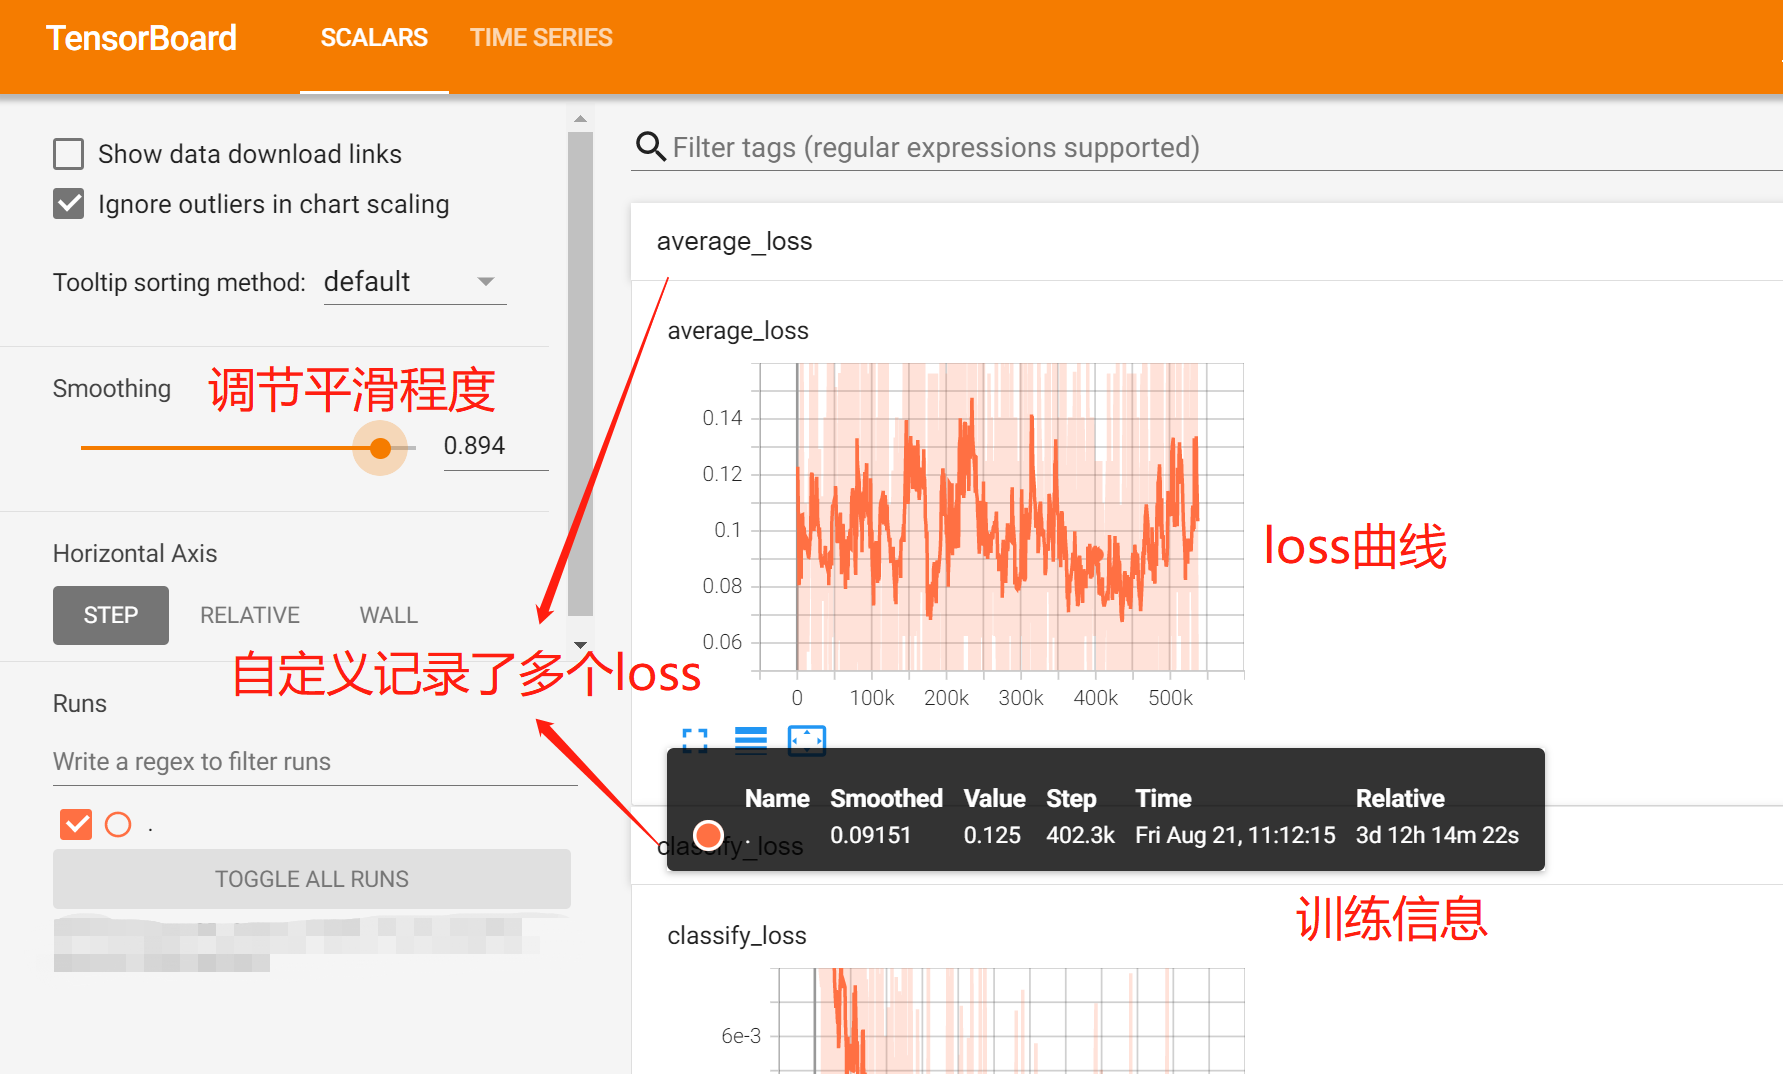
\includegraphics[width=0.8\linewidth]{figures/tensorboard_demo.png}
        % \vspace{-1cm}
        \caption{tensorboard示例图}
        \label{fig:tensorboard_demo}
    \end{center}
    %\vspace{-0.7cm}
\end{figure}

下面介绍具体的封装细节,tb\_logger的初始化和记录代码为:

\begin{minted}[xleftmargin=20pt,linenos,bgcolor=bg]{python}
tb_logger.add_scalar(f'metrics/{metric}', value, current_iter)
#这个是记录validation结果的。
\end{minted}

一个上述语句封装的例子:

\begin{minted}[xleftmargin=20pt,linenos,bgcolor=bg]{python}
#BasicSR/basicsr/train.py中:
    tb_logger = init_tb_loggers(opt)
    #初始化tb_logger
    msg_logger = MessageLogger(opt, current_iter, tb_logger)
    #实例化msg_logger,包含了tb_logger
    ……
    log_vars.update(model.get_current_log())
    #更新log_vars
    msg_logger(log_vars)
    #调用messagelogger

#BasicSR/basicsr/utils/logger.py中定义了MessageLogger类:
    class MessageLogger():
        ……
        def __call__(self, log_vars):
            ……
            self.tb_logger.add_scalar(f'losses/{k}', v, current_iter)
            #这里调用了添加tb_logger
            
#BasicSR/basicsr/models/base_model.py中定义了get_current_log():
    def get_current_log(self):
        return self.log_dict

#self.log_dict在BasicSR/basicsr/models/sr_model.py中:
    loss_dict['l_pix'] = l_pix
    self.log_dict = self.reduce_loss_dict(loss_dict)
\end{minted}

\end{document}